\chapter{Evaluation}
\label{sec:eval}




%\comment{Gad: This is a sketch for the evaluation. We want to evaluate our approach based on the predictions. We are using the full KG as an approximation of an ideal graph and hide 20\% of it to obtain the available graph that we use for learning Horn rules.
%After predicting facts with the mined Horn rules % and input graph:  
%1) we can automatically annotate the predicted facts as true if they exist in the ideal graph
%2) we can automatically annotate the predicted facts as false if they contradict the ideal graph by exploiting functional, disjoint, and asymmetric relations.
%3) If the automatically annotated part is big enough relative to the unkown (e.g. 80:20), we can use it to evaluate our Horn rules and their revisions.
%4) We use the ratio between the facts automatically annotated as true and the facts annotated as false to determine the quality of the mined Horn rules.
%5) The ratio between the removed false predictions and the true predictions will determine the quality of the revisions.}





% OLD Text: >>
%Our revision approach is implemented in Java in a system prototype\footnote{https://github.com/htran010589/nonmonotonic-rule-mining}. We conducted preliminary experiments on a  multi-core Linux server %using 
% with 40 cores and 400GB RAM and evaluated how our revision approach impacts (1) the quality of the rules and (2) the correctness of the predictions they produce. To estimate (1), we compare the average conviction of the Horn rules with their revisions, and measure $q_{\mi{conflict}}$ for the revised ruleset. To evaluate (2), we count the number of true (resp. false) facts that were correctly preserved (resp. neglected) by the revised rules among all Horn rule predictions. 


%<<
Our revision approach aims at enhancing the (i) the quality of the rules and (ii) the correctness and consistency of the predictions they produce. To estimate the first, we compare the average conviction of the Horn rules with their revisions.
%, and measure $q_{\mi{conflict}}$ for the revised ruleset.
While to evaluate the later, we count the number of true facts among all Horn rule predictions that are correctly preserved as well as the erroneous facts that are removed by the revised rules.  

%>>>
% \leanparagraph{Dataset} For the approximation $\cG^i_{appr}$ of the ideal graph we %evaluation %We evaluate our method on a KG 
%  take a KG extracted from the IMDB~\footnote{http://imdb.com} dataset with $111783$ entities, $38$ relations and $583380$ facts~\footnote{https://dl.dropboxusercontent.com/u/12978004/ILP2016\_IMDB\_data.zip}. We constructed the available graph $\cG^a$ with $511482$ facts by removing from $\cG^i_{\mi{appr}}$ 20\% of the facts for each binary predicate. As a side constraint we ensure that in $\cG^a$ every node is connected to at least one other node. 
%<<
\begin{figure}
\centering
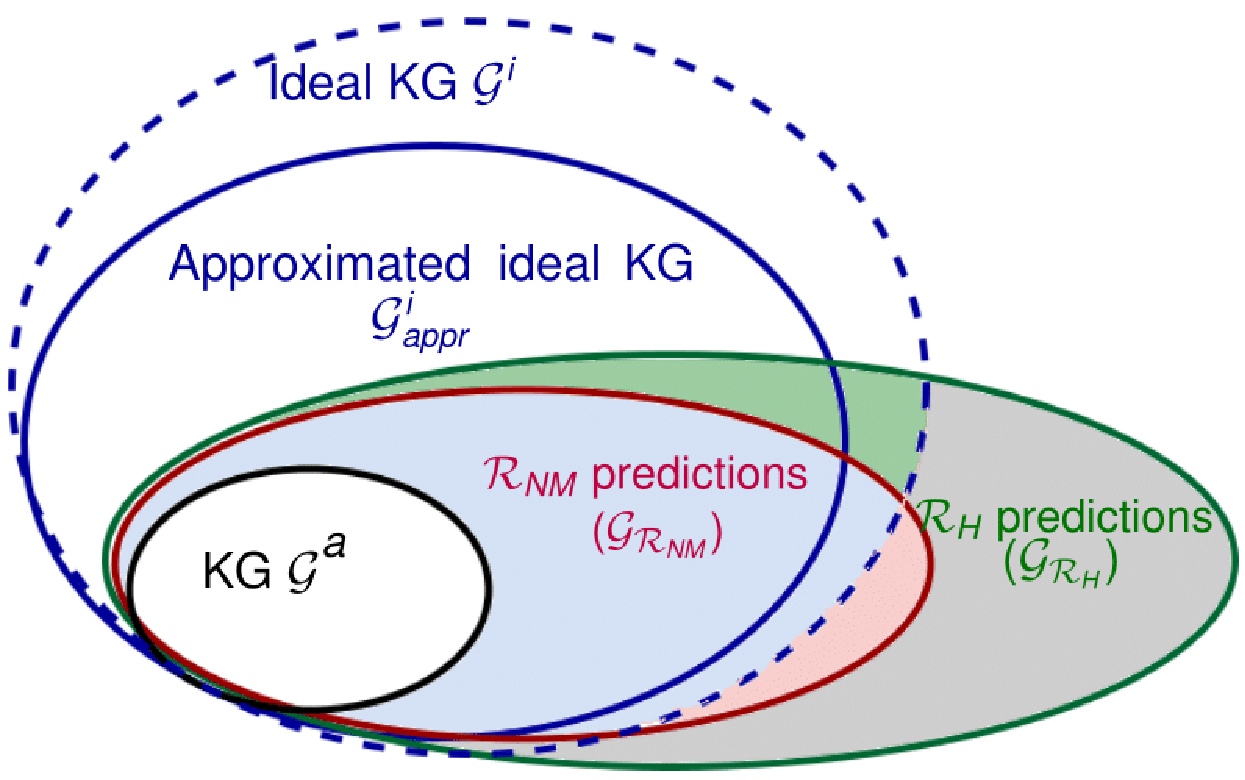
\includegraphics[width=0.5\textwidth]{figures/big_pic_exp}
\caption{Venn diagram shows the relation between the ideal, approximated and available slices of the KG}
\label{fig:venn}
\end{figure}
\leanparagraph{Dataset} In order to automate the evaluation process, we need an ideal graph $\cG^i$ (Fig~\ref{fig:venn}) which is known to be complete as a ground truth. However, obtaining a real life complete KG is not possible. Therefore, we use the existing KG as an approximation $\cG^i_{appr}$ for the ideal graph $\cG^i$. Then, we constructed the available graph $\cG^a$ by removing from $\cG^i_{\mi{appr}}$ 20\% of the facts for each binary predicate. As a side constraint, we ensure that in $\cG^a$ every node is connected to at least one other node. We evaluated our approach on two KGs separately: (i) YAGO3~\cite{yago3}, as general purpose KG with \missing{N} entities and \missing{N} relations, and (ii) a KG extracted from the IMDB~\footnote{http://imdb.com} dataset with $111783$ entities, $38$ relations and $583380$ facts~\footnote{https://dl.dropboxusercontent.com/u/12978004/ILP2016\_IMDB\_data.zip}. 

\leanparagraph{Setup} 
First, the workflow of the experiment starts with mining Horn rules of the form $\mi{h(X,Y)\leftarrow p(X,Z),q(Z,Y)}$ from $\cG^a$ and rank them w.r.t. %the 
\textit{conviction} %measure 
\cite{convict}.
%>>>
% \begin{equation}
% \mi{conv(r)=\dfrac{1-\mi{supp(r)}}{1-\mi{conf(r)}}},
% \end{equation}
% where $\mi{supp(r)}$ and $\mi{conf(r)}$ are resp. the support and the confidence of the rule $r$.
% We use this measure, since it appears to be well-suited for prediction as claimed in \cite{rulemeasures}.
%<<
We then compute three $\mi{EWS}$s{:} $\mi{EWS(r,\cG,X)}${,}$\mi{EWS(r,\cG,Y)}$ and $\mi{EWS(r,\cG,\tuple{X,Y})}$ over the variables appearing in the head of $r$. Revisions of the rule are created by incorporating single exception candidate from one of the three $\mi{EWS}$s. We take conviction as the $\mi{rm}$ function and rank the constructed revisions using one of the proposed ranking methods, namely \emph{Naive}, \emph{OP}, and \emph{OPM}. For every rule $r$, we pick the revision with the highest $\mi{rm}$.
%>>>
%exception out of all exception candidates in the three $\mi{EWS}$s for which the revised rule gets the highest score.\comment{gad: should not that be already in the methodology?}\comment{ds: right, moved}
%<<<

%\vspace{-1.2cm}
\leanparagraph{Ruleset quality results} 
In Table~\ref{tab:rules_quality}, we report the average conviction for the top-$\mi{k}$ ($k=5,10,15,20$) revised rules using the different ranking methods and their Horn versions $\cR_{H}$ for both YAGO and IMDB. 

% The second and the third columns contain average conviction for $\cR_{\mi{H}}$ and $\cR_{\mi{NM}}$ resp., while the  fourth column stores the value of $\mi{q_{\mi{conflict}}(\cR_{NM},\cG^a)}$ as defined in Eq.~\ref{eq:conflict}. 
The results show that the revision process consistently enhanced the average conviction. For YAGO the highest increase is \missing{n} in the case of the top-\missing{k}, while in IMDB, it is \missing{n} for the top-\missing{k}.

\leanparagraph{Predicted facts quality}

Table~\ref{prediction_res} contains the predicates that result from applying top-\missing{k} revised rules. First, we report the prediction results of applying the rulesets $\cR_{\mi{H}}$ and $\cR_{\mi{OPM}}$ separately on $\cG^a$ using the DLV system~\cite{dlv} to generate the extended graphs. In addition, we use the auxiliary set of rules $\cR_{\mi{OPM}}^{\mi{aux}}$ along with  $\cR_{\mi{OPM}}$ to measure the conflicts.

%\comment{GAD: to be continued here .. more about the table}

%>>
% The last five columns present the prediction results of applying the rulesets $\cR_{\mi{H}}$ and $\cR_{\mi{NM}}$ on $\cG^a$ using the DLV system~\cite{dlv} to generate the extended graphs $\cG^a_{\cR_H}$ and $\cG^a_{\cR_{NM}}$ respectively.

% Here, ``\textbf{all}'' refers to the number of all predictions produced by the rulesets, and ``\textbf{in $\cG^i_{\mi{appr}}$}" stores the number of predictions in the approximation of the ideal graph. Among the rest of the predicted facts outside $\cG^i_{\mi{appr}}$, in ``\textbf{corr. negl.}" we count the number of erroneous predictions made by $\cR_{H}$, that were \textbf{correctly neglected} by $\cR_{\mi{NM}}$. Since these predictions are not present in the original KG, we had to assess them manually by consulting such Web resources as Wikipedia and IMDB.
%<<

Overall, we were able to predict 5278 facts using the top-20 Horn rules, from which 16\% can be verified from $\cG^i_{\mi{appr}}$. Since the Horn versions  of the top-5 rules are already of a high quality, their revisions did not prevent erroneous predictions. With the increase of the number of the considered rules, the percentage of the false facts correctly neglected %erroneous predictions prevented 
by our revised rules increases  reaching 67\% for the top-20 rules. 
%Note that in the current experiments the truthfulness of predictions outside $\cG^i_{\mi{appr}}$ made both by $\cR_{\mi{H}}$ and $\cR_{\mi{NM}}$ is not estimated due to the large number of facts to be manually checked. 
In the future work we plan to semi-atomatically derive the truthfulness of the unknown facts outside $\cG^i_{\mi{appr}}$ predicted both by $\cR_{\mi{H}}$ and $\cR_{\mi{NM}}$ exploiting  properties like (a)symmetry or transitivity of the relational predicates as well as making use of information extraction techniques. % compared to the predictions made by $\cR_{H}$.

For the 134 Horn rules mined from $\cG^a$ all $\mi{EWS}$s with an average of 1649 exception candidates for each rule were computed within 10 sec. The overall best revision for 134 Horn rules was determined in 30 sec., and the predictions using the revised top-$k$ rules on $\cG^a$ were found whithin 1.5 min. via the DLV system. 

 %till the top-15 rules because the number of predictions is increasing while the rules are still independent.
%\comment{DS: decreases with the growing k; one needs to explain why?, Gad: Do you think it is better now?} 
%Then, a rule in the top-20 rules caused more conflicts which explains the slight increase to 13\%. 

%\begin{table}[t]
%\centering
%\footnotesize
%\renewcommand*{\arraystretch}{1.07}
%


\footnotesize{
\resizebox{\columnwidth}{!}{%

\begin{tabular}{|l|llll|llll|llll|}
\hline
       \multirow{2}{*}{\textbf{\textit{topk}}}                    & \multicolumn{4}{c|}{\textbf{YAGO}}        & \multicolumn{4}{c|}{\textbf{IMDB}}  & \multicolumn{4}{c|}{\textbf{Sample WIKIDATA}}      \\ \cline{2-13} 
       %\hline
 & $\cR_{H}$ & $\cR_{N}$ & $\cR_{PM}$ & $\cR_{OPM}$ & $\cR_{H}$ & $\cR_{N}$ & $\cR_{PM}$ & $\cR_{OPM}$ & $\cR_{H}$ & $\cR_{N}$ & $\cR_{PM}$ & $\cR_{OPM}$ \\ \hline
5   & 1.3784 & 1.3821 & 1.3821 & 1.3821 & 2.2670 & 2.3014 & 2.3008 & 2.3014 & 3.2282 & 3.2342 & 3.2340 & 3.2342\\ %\hline
30   & 1.1207 & 1.1253 & 1.1236 & 1.1237 & 1.5453 & 1.5644 & 1.5543 & 1.5640 & 3.1118 & 3.4315 & 3.4194 & 3.4271\\ %\hline
50   & 1.0884 & 1.0923 & 1.0909 & 1.0913 & 1.3571 & 1.3749 & 1.3666 & 1.3746  & 2.7115 & 2.9193 & 2.9070 & 2.9135\\ %\hline
60   & 1.0797 & 1.0837 & 1.0823 & 1.0829 & 1.3063 & 1.3221 & 1.3143 & 1.3219  & 2.4930 & 2.7101 & 2.6986 & \textbf{2.7046}\\ %\hline
70   & 1.0714 & 1.0755 & 1.0736 & 1.0744 & 1.2675 & 1.2817 & 1.2746 & 1.2814  & 2.3395 & 2.5272 & 2.3931 & 2.5219\\ %\hline
80   & 1.0685 & 1.0731 & 1.0710 & 1.0720 & 1.2368 & 1.2499 & 1.2431 & 1.2497  & 2.4071 & 2.5781 & 2.4597 & 2.5734\\ %\hline
100   & 1.0618 & 1.0668 & 1.0648 & 1.0659 & 1.3074 & 1.4100 & 1.3987 & 1.4098  & 2.3258 & 2.4847 & 2.3859 & 2.4806\\ \hline

\end{tabular}

}
}

% \centering
% \caption{My caption}
% \label{my-label}
% \begin{tabular}{l|l|l|l|l|l|l|l|l|}
% \cline{2-9}
%                            & \multicolumn{4}{c|}{YAGO manual}        & \multicolumn{4}{c|}{IMDB top rules}        \\ \hline
% \multicolumn{1}{|l|}{\textit{topk}} & $\cR_{H}$ & $\cR_{N}$ & $\cR_{PM}$ & $\cR_{OPM}$ & $\cR_{H}$ & $\cR_{N}$ & $\cR_{PM}$ & $\cR_{OPM}$ \\ \hline
% \multicolumn{1}{|l|}{5}    &   1.10    &   1.11    &    1.20    &    1.15     &   2.27    &   2.3    &   2.89     &  2.55       \\ \hline
% \multicolumn{1}{|l|}{10}   &    1.10   &   1.11    &    1.23    &    1.18     &   1.9    &   1.92    &    4.74    &  2.07       \\ \hline
% \multicolumn{1}{|l|}{15}   &   1.12    &   1.13    &    1.32    &    1.18     &   1.8    &   1.82    &   5.25     &   1.98      \\ \hline
% \multicolumn{1}{|l|}{20}   &       &       &        &         &       &       &        &         \\ \hline
% \end{tabular}

%\medskip
%\caption{Rule revision results}
%\label{tab:rules_quality}
%\end{table}
%
%
%\begin{table}[]
%\centering
%
% \begin{tabular}{c|l|llll|llll}
% \hline
%  \multirow{2}{*}{}              &   \multirow{2}{*}{\textbf{$\mi{head(r)}$}}   	& \multicolumn{4}{c|}{\textbf{predictions}} 						&  \multicolumn{4}{c}{\textbf{outside $\cG^i_{appr}$}}  				\\ \cline{3-10} 
%          						&  									& $\cR_\mi{H}$  & $\cR_{N}$ & $\cR_{PM}$  		& $\cR_{OPM}$ &  $\cR_\mi{H}$     & $\cR_{\mi{N}}$ 	& $\cR_\mi{PM}$     & $\cR_{\mi{OPM}}$    \\ \hline
% %\multirow{4}{*}{\rotatebox{90}{YAGO}}
% & directed & 41079 & 39174 & 39174 & 39174  & 41021 & 39116 & 39116 & 39116 \\ %\cline{2-10}
%  & gradFrom & 3519 & 3456 & 3456 & 3456  & 3363 & 3300 & 3300 & 3300 \\ %\cline{2-10}
%  & citizenOf & 3407 & 2883 & 2883 & 2883  & 3360 & 2836 & 2836 & 2836 \\ %\cline{2-10}
%  & bornIn & 110283 & 108317 & 109846 & 108317 & 109572 & 107607 & 109137 & 107607 \\ \hline\hline %\cline{1-10}
% %\multirow{4}{*}{\rotatebox{90}{IMDB}} 
% & actIn & 1231 & 1214 & 1230 & 1214 & 1148 & 1131 & 1147 & 1131 \\ %\cline{2-10}
%  & genre & 629 & 609 & 618 & 609  & 493 & 477 & 482 & 477 \\% \cline{2-10}
%  & hasLang & 173 & 102 & 125 & 102 & 163 & 92 & 115 & 92 \\ %\cline{2-10}
%  & prodIn & 2489 & 2256 & 2327 & 2327 & 2488 & 2255 & 2326 & 2326 \\ \cline{1-10}
% \end{tabular}
\footnotesize{
\resizebox{\columnwidth}{!}}}  				\\ \cline{2-12} 
 		& $\cR_\mi{H}$  & $\cR_{\mi{N}}$ & $\cR_{\mi{PM}}$  		& $\cR_{\mi{OPM}}$ &  $\cR_\mi{H}$     & $\cR_{\mi{N}}$ 	& $\cR_\mi{PM}$     & $\cR_{\mi{OPM}}$  & $\cR_{\mi{N}}$ 	& $\cR_\mi{PM}$     & $\cR_{\mi{OPM}}$   \\ \hline

%\multirow{4}{*}{\rotatebox{90}{IMDB}} 
 $\mi{{I}{:}{actedIn}}$ & 1231 & 1214 & 1230 & 1214 & 1148 & 1131 & 1147 & 1131 &90 & 100 & 90\\ %\cline{2-10}
 $\mi{{I}{:}{genre}}$ & 629 & 609 & 618 & 609  & 493 & 477 & 482 & 477 &50 & 20 & 50\\% \cline{2-10}
 $\mi{{I}{:}{hasLang}}$ & 173 & 102 & 125 & 102 & 163 & 92 & 115 & 92 &  60 & 100 & 60\\ %\cline{2-10}
 $\mi{{I}{:}{prodIn}}$ & 2489 & 2256 & 2327 & 2327 & 2488 & 2255 & 2326 & 2326 & 10 & 10 & 30 \\ \cline{10-12}
 &  &  &  &  &  &  &  &  	& 52.50  & 45.16   & \textbf{57.75}  \\
\hline 
$\mi{{Y}{:}{direct}}$ & 41079 & 39174 & 39174 & 39174  & 41021 & 39116 & 39116 & 39116 & 100 & 100 & 100   \\
 $\mi{{Y}{:}{grFrom}}$ & 3519 & 3456 & 3456 & 3456  & 3363 & 3300 & 3300 & 3300 & 100 & 100 & 70 \\ 
 $\mi{{Y}{:}{citizOf}}$ & 3407 & 2883 & 2883 & 2883  & 3360 & 2836 & 2836 & 2836 & 50 & 50 & 70 \\ 
 $\mi{{Y}{:}{bornIn}}$ & 110283 & 108317 & 109846 & 108317 & 109572 & 107607 & 109137 & 107607 &90& 90 & 100 \\ \cline{10-12}  
 &  &  &  &  &  &  &  &  	& 85  & 85   & 85 \\
 \hline 
 \end{tabular}}}

%\label{prediction_res}
%\end{table}



\begin{figure}[tb]
    \centering
   
    \vspace{-.5cm}
    \begin{tabular}{l}
 {\scriptsize
        %\multirow{6}{*}{YAGO $\begin{cases} \\ \\ \end{cases}$}
        $r_1:  \mi{writtenBy(X, Z)}  \leftarrow
        \mi{hasPredecessor(X, Y)},\mi{writtenBy(Y, Z)},$ $ \textbf{not}$  $\mi{is\_American\_film(X)} $}\\        
       {\scriptsize 
$r_2:  \mi{actedIn(X, Z)}  \leftarrow
        \mi{isMarriedTo(X, Y)},\mi{directed(Y, Z)},$ $ \textbf{not}$  $\mi{is\_silent\_film\_actor(X)} $} \\
       {\scriptsize
                        $r_3:  \mi{bornIn(X, Z)}  \leftarrow
        \mi{direct(X, Y)},\mi{producedIn(Y, Z)},$ $ \textbf{not}$ $\mi{is\_American\_film\_director(X)}$     } \\
 \end{tabular}            
    \caption{Examples of the revised rules}
 \label{fig:examplerules}
 \vspace{-.4cm}
\end{figure}




Fig.~\ref{fig:examplerules} shows examples for our revised rules, e.g., $\mi{r_1}$ states that the writers of movie plots stay the same throughout the sequel with the exception of American movies. %is the same as the writer of its predecessor, %which  is indeed true for most of the cases but not always. 
%unless the movie is American. 
%Indeed, the latter often do not follow the above pattern, for instance the story writer of Batman changes from version to version. %Our revised version excluded American movies which may not follow the general rule, e.g. Batman Movie, the story writer changes from serie to serie. 
The Horn version of $\mi{r_2}$ reflects that the movie directors normally have their spouses on the cast. Our revision approach excluded the old silent movies, for which this practice was not common.










%\ju{The results are not so good :( Of 70K facts that you removed from IMDB, you only managed to re-infer 5K. The errors that you removed are 157 in the best case, which means that only 3\% of the of the Horn predictions are false. Did you investigate on the exceptions/removed facts? My feeling is that they come only from some specific sources. In other words, probably only very few rules of the top 20k get good revisions which remove errors. What you can stress, in order to highlight more the positive results, is to mention that 75\% of the 232 (=5278-5046) removed facts is something wrong. It is not clear how you detected these are mistakes. Are these facts not appearing in the 20\% that you removed or are facts that you manually checked? This should be clarified.}

%\ju{Another point is that I would remove the top5K. You only derived 345 facts, which are not many. You should also try with top-100,1000 but I guess there is no time for that.}




%The quality of the revised rulesets can be evaluated \wrt\ the overall enhancement in the average quality and conflict ratio as discussed in~\cite{iswc2016}. However, in this work we focus on evaluating the quality of the final predictions. That is, we aim at measuring the distance between $\cG^i$ and $\cG_{\cR_H}$ and comparing it to the distance between $\cG^i$ and $\cG_{\cR_{*}}$ for $*\in \{\mi{N,PM,OPM}\}$. 

% We then construct revised rules by picking for every $r\in \cR_H$ exception that 

%We then calculate implemented a simple inductive learning
%procedure to calculate the $\mi{EWS}$s. For each rule we learn three independent $\mi{EWS}$s, one for each variable in the head atom and one for the binary relation between them. Each $\mi{EWS}$ is ranked independently as described in Sec.~\missing{secNum}. We could find $\mi{EWS}$s for \missing{n} rules mined from $\cG^{in}$. On average, the $\mi{EWS}$s rules contained \missing{x} exceptions. To facilitate comparison, we create one revision for each rule using the best exception candidate from the three $\mi{EWS}$s. 

%\leanparagraph{Revisions Quality} 
% Therefore, 
%We create the completions $\cG^a_{\cR_H}, \cG^a_{\cR_N}, \cG^a_{\cR_{PM}}$ and $\cG^a_{\mi{OPM}}$ of $\cG^a$ %used $\cG^{a}$ along with 
%respectively 
%using the DLV system~\cite{dlv}. The four obtained graphs are compared to the approximation of the $\cG^i$. % to assess the correctness of the predicted facts. The assessment is divided into: 
%\begin{enumerate*}[label=(\itshape\roman*\upshape)]
%\item Predicted facts that exist in $\cG^i$ are annotated as true predictions.
%\item Predicted facts that contradict $\cG^i$ are annotated as false predictions. The knowledge about the functional, asymmetric, and disjoint relations is exploited to capture the contradictions, e.g. $\mi{parent(X,Y)}$ and $\mi{hasChild(X,Y)}$ cannot hold for the same pair. 
%\item Remaining facts are sampled and assessed manually based on the Web search results. %by checking the data from the web.
%\end{enumerate*}


%\begin{table}[tb]
%\centering

% \begin{tabular}{@{}l|l|l|l|l|l@{}}
% \toprule
%      & Total predictions & In $\cG_i$ & Contradicts $\cG_i$ & Manually True & Manually False \\ \midrule
% Horn &             &            &                    &               &                \\
% PM   &             &            &                    &               &                \\
% OPM  &             &            &                    &               &                \\ \bottomrule
% \end{tabular}

% Please add the following required packages to your document preamble:
% \usepackage{booktabs}

% older version of the table
%\begin{tabular}{@{}l|ll|ll|ll|cl|cl@{}}
%\toprule
%   & \multicolumn{2}{c|}{Avg. Conv.}                & \multicolumn{2}{c|}{\;\;Predictions\;\;}                    & \multicolumn{2}{c|}{In $\cG^{i}$}                   & \multicolumn{2}{c|}{Conflicts}  & \multicolumn{2}{l|}{Corr. Rem.} \\ \cmidrule(l){2-11} 
%   & \multicolumn{1}{c}{Horn} & \multicolumn{1}{c|}{NM} & \multicolumn{1}{c}{Horn} & \multicolumn{1}{c|}{NM} & \multicolumn{1}{c}{Horn} & \multicolumn{1}{c|}{NM} & Horn & \multicolumn{1}{c|}{NM} & Horn     & \multicolumn{1}{c}{NM}     \\ \midrule
%5  &  4.08                     &                        6.16 &            345 \;\;\;\;             &            331              &  161                        &                        156  & -    &  0.28                        & -        &                             \\
%10 &  2.91                        &                        4.21  &           2178               &             2118             &  456                        &                        450  & -    &  0.08                        & -        &                             \\
%15 &  2.5                        &                      3.42    &           3482               &            3348              &  629                        &                        622  & -    &  0.09                        & -        &                             \\
%20 &  2.29                        &                        3.0  &             5278             &           5046               &  848                        &                        835  & -    &  0.13                        & -        &        71.69                    \\ \bottomrule
%\end{tabular}
%\caption{Results of applying different rule revisions on $\cG_{in}$}
%\label{tab:predicton_results}
%\end{table}
